\documentclass{article}
\usepackage[english]{babel}
\usepackage[utf8]{inputenc}
\usepackage[T1]{fontenc}

\usepackage{amsmath} % math stuff
\usepackage{amssymb} % math stuff
\usepackage{amsthm}  % math stuff
\usepackage{commath} % math stuff
\usepackage{relsize} % math stuff
\usepackage{caption} % caption stuff
\usepackage{fancyhdr} % custom headers
\usepackage{lastpage} % determine last page for the footer
\usepackage{extramarks} % headers and footers
\usepackage{graphicx} % images
\usepackage{listings} % code listings
\usepackage{courier} % courier font
\usepackage{enumerate}
\usepackage{enumitem}
\usepackage{mathtools}
\usepackage{titling}
\usepackage{float}
\usepackage{cite}
\usepackage[mathscr]{eucal}
\usepackage{subcaption}
\usepackage{marvosym}
\usepackage{makecell}

\usepackage{pgfplots}
\pgfplotsset{
  every axis plot/.append style={line width=0.8pt},
  compat=1.17,
}

%tikz
\usepackage{tikz}
\usetikzlibrary{arrows}
\usetikzlibrary{positioning}

\newcommand{\given}{\,\middle|\,}

\title{Getting robots bored enough to move cubes}
\author{Julien Scholz}
\date{\today}

\begin{document}

\begin{titlepage}
    \centering
    University of Hamburg \par
    MIN Faculty \par
    Department of Informatics \par
    BSc Informatics \par
    \vspace{6\baselineskip}
    {\Large Bachelor's Thesis\par}
    {\Huge \thetitle \par}
    \vspace{6\baselineskip}
    by\par
    {\Large \theauthor \par 7065721 \par}
    \vfill
    Thesis advisors:\par
    {\large Dr. Cornelius Weber, \par Dr. Muhammad Burhan Hafez}
\end{titlepage}

\begin{abstract}
    \noindent
    Using a model of the environment, reinforcement learning agents can plan their future moves and achieve super-human performance in board games like Chess, Shogi, and Go, while remaining relatively sample efficient. As demonstrated by the MuZero Algorithm, the environment model can even be learned dynamically, generalizing the agent to many more tasks while at the same time achieving state-of-the-art performance. Notably, MuZero uses internal state representations instead of real environment states for its predictions. In this thesis, we introduce two additional, independent loss terms to MuZero's overall loss function, which work entirely unsupervised and act as constraints to stabilize the learning process. Experiments show that they provide a significant performance increase in simple \mbox{OpenAI Gym} environments. Our modifications also enable self-supervised pretraining for MuZero, meaning the algorithm can learn about environment dynamics before a goal is made available.
\end{abstract}

\vspace{1cm}

\renewcommand{\abstractname}{Zusammenfassung}
\begin{abstract}
    \noindent
    Mithilfe eines Modells der Umgebung können Reinforcement Learning Agenten vorausplanen, und so beispielsweise Menschen in Brettspielen wie Schach, Shōgi und Go schlagen, ohne dafür viele Trainingsbeispiele zu benötigen. Insbesondere hat der MuZero Algorithmus bestätigt, dass das Modell durch Interaktion mit der Umgebung erlernt werden kann (und somit nicht bereitgestellt werden muss) ohne dabei die herausragenden Ergebnisse zu beeinträchtigen. MuZero verwendet hierfür interne Repräsentationen der Umgebungszustände. In dieser Bachelorthesis beschreiben wir zwei zusätzliche Loss-Terme, welche vollständig unüber\-wacht funktionieren, und MuZeros Loss-Funktion beigefügt werden können um den Lernprozess zu stabilisieren. Experimentell können wir so eine Verbesserung der Leistung in einfachen OpenAI Gym Umgebungen zeigen. Zusätzlich erlauben die Änderungen, dass der MuZero Agent die Mechaniken seiner Umgebung bereits vor Einführung eines Ziels erlernen kann.
\end{abstract}

\vfill

\begin{center}
    Note: Figures that do not include a citation were drawn by the author.
\end{center}

\tableofcontents

\section{Introduction}
The field of artificial intelligence has become increasingly popular over the past years.
\section{Background}

\subsection{Reinforcement Learning}

\begin{frame}[fragile]{Markov Decision Process}
    \begin{figure}
        \centering
        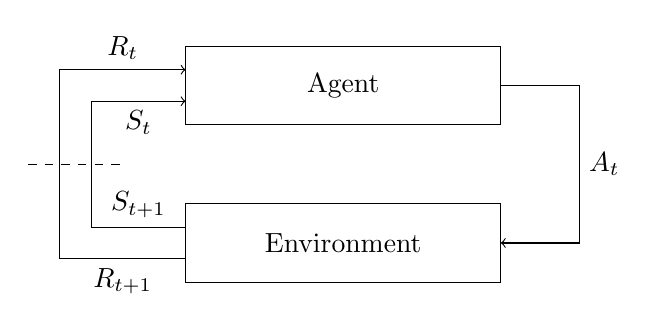
\begin{tikzpicture}
            \draw (0, 2) rectangle node {Agent} (4, 3);
            \draw (0, 0) rectangle node {Environment} (4, 1);

            \draw [->] (4, 2.5) -- (5, 2.5) -- node[right] {$A_t$} (5, 0.5) -- (4, 0.5);

            \draw [->] (0, 0.3) -- node[below] {$R_{t+1}$} (-1.6, 0.3) -- (-1.6, 2.7) --node[above] {$R_t$}  (0, 2.7);
            \draw [->] (0, 0.7) -- node[above] {$S_{t+1}$} (-1.2, 0.7) -- (-1.2, 2.3) -- node[below] {$S_t$} (0, 2.3);

            \draw [dashed] (-2, 1.5) -- (-0.8, 1.5);
        \end{tikzpicture}
        \caption{The agent-environment feedback loop in a Markov Decision Process. \cite{bible}}
        \label{fig:mdp_visualization}
    \end{figure}
\end{frame}

\begin{frame}{Policies and Values}
    \begin{itemize}
        \item Goal of an agent: Maximize \textit{return} (sum of future rewards)
        \item Behavior of an agent to reach the goal is called \textit{policy}
        \item \textit{Value} $v_\pi(s)$ is the expected return when following policy $\pi$ in state $s$
        \item Policies and value functions are usually constructed from neural networks
    \end{itemize}
\end{frame}

\begin{frame}[fragile]{Model-Based Reinforcement Learning}
    \begin{figure}
        \centering
        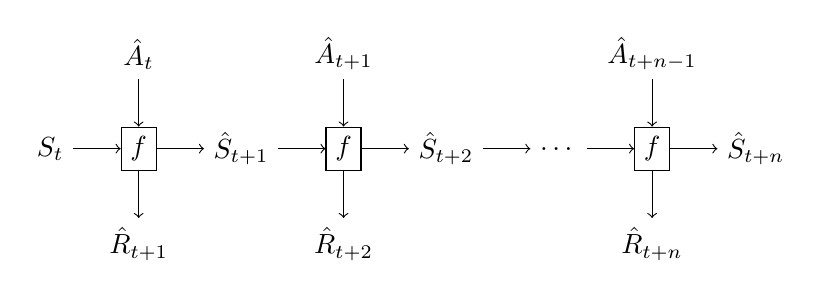
\begin{tikzpicture}[node distance=0.6]
            \node (St) {$S_t$};

            \node [right = of St, draw, rectangle] (f1) {$f$};
            \node [above = of f1] (At) {$\hat{A}_t$};
            \node [below = of f1] (Rtp1) {$\hat{R}_{t+1}$};

            \node [right = of f1] (Stp1) {$\hat{S}_{t+1}$};

            \onslide<2->{
                \node [right = of Stp1, draw, rectangle] (f2) {$f$};
                \node [above = of f2] (Atp1) {$\hat{A}_{t+1}$};
                \node [below = of f2] (Rtp2) {$\hat{R}_{t+2}$};

                \node [right = of f2] (Stp2) {$\hat{S}_{t+2}$};

                \node [right = of Stp2] (dots) {$\dots$};

                \node [right = of dots, draw, rectangle] (f3) {$f$};
                \node [above = of f3] (Atpnm1) {$\hat{A}_{t+n-1}$};
                \node [below = of f3] (Rtpn) {$\hat{R}_{t+n}$};

                \node [right = of f3] (Stpn) {$\hat{S}_{t+n}$};
            }

            \draw [->] (St) -- (f1);
            \draw [->] (At) -- (f1);
            \draw [->] (f1) -- (Rtp1);
            \draw [->] (f1) -- (Stp1);

            \onslide<2->{
                \draw [->] (Stp1) -- (f2);
                \draw [->] (Atp1) -- (f2);
                \draw [->] (f2) -- (Rtp2);
                \draw [->] (f2) -- (Stp2);

                \draw [->] (Stp2) -- (dots);
                \draw [->] (dots) -- (f3);

                \draw [->] (Atpnm1) -- (f3);
                \draw [->] (f3) -- (Rtpn);
                \draw [->] (f3) -- (Stpn);
            }
        \end{tikzpicture}
        \caption{An environment model $f$ being applied recursively to predict the outcome of a trajectory. \nocite{bible, model}}
        \label{fig:recursive_model}
    \end{figure}
\end{frame}

\begin{frame}{Use Cases of Model-Based RL}
    \begin{figure}
        \centering
        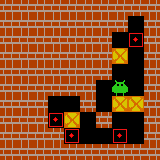
\includegraphics[width=0.5\textwidth]{assets/sokoban.png}
        \caption{Screenshot of the puzzle video game Sokoban. \cite{sokoban}}
        \label{fig:sokoban}
    \end{figure}
\end{frame}

\subsection{MuZero Algorithm}

\begin{frame}[fragile]{MuZero Algorithm}
    \begin{figure}
        \centering
        \begin{tikzpicture}[node distance=0.5]
            \node (ot) {$o_t$};
            \node [left = of ot] (otm1) {$o_{t-1}$};
            \node [right = of ot] (otp1) {$o_{t+1}$};
            \node [left = of otm1] (otm2) {$\dots$};
            \node [right = of otp1] (otp2) {$\dots$};
            \draw [->, dashed] (otm2) -- (otm1);
            \draw [->, dashed] (otm1) -- (ot);
            \draw [->, dashed] (ot) -- (otp1);
            \draw [->, dashed] (otp1) -- (otp2);

            \pause

            \node [below = of ot, draw] (h) {$h_\theta$};
            \node [below = of h] (s0) {$s^0$};
            \draw [->] (ot) -- (h);
            \draw [->] (h) -- (s0);

            \pause

            \node [right = of s0, draw] (g0) {$g_\theta$};
            \node [right = of g0] (s1) {$s^1$};
            \node [above = of g0] (a1) {$a^1$};
            \node [below = of g0] (r1) {$r^1$};
            \draw [->] (s0) -- (g0);
            \draw [->] (a1) -- (g0);
            \draw [->] (g0) -- (s1);
            \draw [->] (g0) -- (r1);

            \node [right = of s1, draw] (g1) {$g_\theta$};
            \node [right = of g1] (s2) {$s^2$};
            \node [above = of g1] (a2) {$a^2$};
            \node [below = of g1] (r2) {$r^2$};
            \draw [->] (s1) -- (g1);
            \draw [->] (a2) -- (g1);
            \draw [->] (g1) -- (s2);
            \draw [->] (g1) -- (r2);

            \node [right = of s2, draw] (g2) {$g_\theta$};
            \node [right = of g2] (s3) {$s^3$};
            \node [above = of g2] (a3) {$a^3$};
            \node [below = of g2] (r3) {$r^3$};
            \draw [->] (s2) -- (g2);
            \draw [->] (a3) -- (g2);
            \draw [->] (g2) -- (s3);
            \draw [->] (g2) -- (r3);

            \pause

            \node [below = of s3, draw] (f) {$f_\theta$};
            \node [below = of f] (pv) {$\policy^3, v^3$};
            \draw [->] (s3) -- (f);
            \draw [->] (f) -- (pv);
        \end{tikzpicture}
        \caption{Testing a single action sequence made up of three actions $a^1$, $a^2$, and $a^3$ to plan based on observation $o_t$ using all three MuZero functions. \nocite{muzero}}
        \label{fig:muzero_basic_policy}
    \end{figure}
\end{frame}

\begin{frame}{MuZero's Loss Function}
    \begin{equation*}
        l_t(\theta) = \sum^K_{k=0} \left(l^r(u_{t+k}, r_t^k) + l^v(z_{t+k}, v_t^k) + l^p(\pi_{t+k}, \policy_t^k) + c||\theta||^2\right)
    \end{equation*}
    \begin{itemize}
        \item Each model output has its own loss term
        \item The model is unrolled through time during training
    \end{itemize}
\end{frame}

\begin{frame}[fragile]{Monte-Carlo Tree Search}
    \begin{figure}
        \centering
        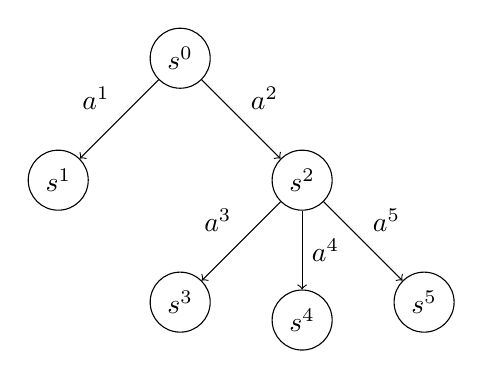
\begin{tikzpicture}
            \node [draw, circle] (s0) {$s^0$};

            \pause

            \node [draw, circle, below left = of s0] (s1) {$s^1$};
            \node [draw, circle, below right = of s0] (s2) {$s^2$};
            \draw [->] (s0) -- node[above left] {$a^1$} (s1);
            \draw [->] (s0) -- node[above right] {$a^2$} (s2);

            \pause

            \node [draw, circle, below left = of s2] (s3) {$s^3$};
            \node [draw, circle, below = of s2] (s4) {$s^4$};
            \node [draw, circle, below right = of s2] (s5) {$s^5$};
            \draw [->] (s2) -- node[above left] {$a^3$} (s3);
            \draw [->] (s2) -- node[right] {$a^4$} (s4);
            \draw [->] (s2) -- node[above right] {$a^5$} (s5);
        \end{tikzpicture}
        \caption{A simplified view of a Monte-Carlo search tree. Note that the number of available actions in state $s^0$ differs from those in state $s^2$. \nocite{mcts}}
        \label{fig:mcts_simple}
    \end{figure}
\end{frame}

\section{Proposed Methods}
In this section, we propose two changes to the MuZero algorithm that may improve its performance. These changes are based on the idea that MuZero is very unconstrained in its embedded state representations, which, while making the algorithm very flexible, may harm the learning process.

Our changes extend MuZero by individually weightable loss terms, meaning they can be viewed as a generalization of the regular MuZero algorithm and may be used either independently or in combination.

\newcommand{\reconstruction}{h^{-1}}

\subsection{Reconstruction Function}
For our first proposed change, we introduce an additional $\theta$-parameterized function, which we call the \textit{reconstruction} function $\reconstruction_\theta$. Whereas the representation function $h_\theta$ maps observations to internal states, the reconstruction function shall perform the inverse operation, that is, mapping internal states to real observations, thereby performing a generative task. Notably, since we are using function approximation, reconstructed observations are unlikely to be perfectly accurate. Moreover, in the probable case that the embedded states store less information than the real observations, it becomes theoretically impossible for $\reconstruction_\theta$ to restore what has been discarded by the representation function. We call $\hat{o}^k_t = \reconstruction_\theta(s^k_t)$ the reconstructed observation for the embedded state $s^k_t$, meaning it is an estimate of the real observation $o_{t+k}$ (see Figure \ref{fig:reconstruction_function}), given that the action sequences given to the environment and the dynamics function are the same.
\afterpage{
    \begin{figure}[t]
        \centering
        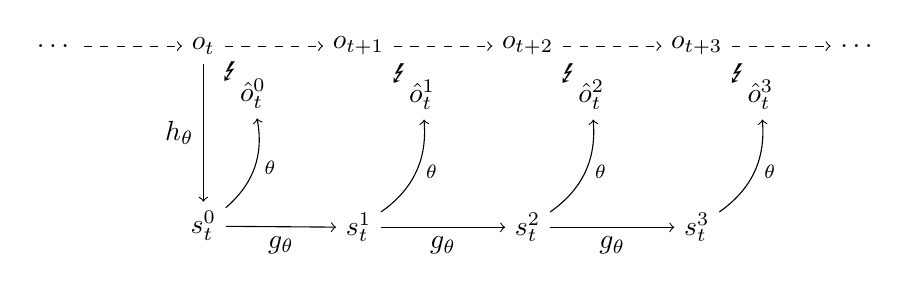
\begin{tikzpicture}[node distance=1.25]
            \node (ot) {$o_t$};
            \node [left = of ot] (otm1) {$\dots$};
            \node [right = of ot] (otp1) {$o_{t+1}$};
            \node [right = of otp1] (otp2) {$o_{t+2}$};
            \node [right = of otp2] (otp3) {$o_{t+3}$};
            \node [right = of otp3] (otp4) {$\dots$};
            \draw [->, dashed] (otm1) -- (ot);
            \draw [->, dashed] (ot) -- (otp1);
            \draw [->, dashed] (otp1) -- (otp2);
            \draw [->, dashed] (otp2) -- (otp3);
            \draw [->, dashed] (otp3) -- (otp4);

            \node [below = 1.75 of ot] (s0) {$s^0_t$};
            \node [below = 1.75 of otp1] (s1) {$s^1_t$};
            \node [below = 1.75 of otp2] (s2) {$s^2_t$};
            \node [below = 1.75 of otp3] (s3) {$s^3_t$};
            \draw [->] (ot) -- node [left] {$h_\theta$} (s0);
            \draw [->] (s0) -- node [below] {$g_\theta$} (s1);
            \draw [->] (s1) -- node [below] {$g_\theta$} (s2);
            \draw [->] (s2) -- node [below] {$g_\theta$} (s3);

            \node [below right = 0.1 of ot] (notot) {$\hat{o}^0_t$};
            \node [below right = 0.1 of otp1] (nototp1) {$\hat{o}^1_t$};
            \node [below right = 0.1 of otp2] (nototp2) {$\hat{o}^2_t$};
            \node [below right = 0.1 of otp3] (nototp3) {$\hat{o}^3_t$};
            \node [below right = -0.2 of ot] {\Lightning};
            \node [below right = -0.2 of otp1] {\Lightning};
            \node [below right = -0.2 of otp2] {\Lightning};
            \node [below right = -0.2 of otp3] {\Lightning};

            \draw [->] (s0) edge [bend right] node [right] {$\reconstruction_\theta$} (notot);
            \draw [->] (s1) edge [bend right] node [right] {$\reconstruction_\theta$} (nototp1);
            \draw [->] (s2) edge [bend right] node [right] {$\reconstruction_\theta$} (nototp2);
            \draw [->] (s3) edge [bend right] node [right] {$\reconstruction_\theta$} (nototp3);
        \end{tikzpicture}
        \caption{The reconstruction function $\reconstruction_\theta$ being used to predict future observations $o_{t+k}$ from internal states $s^k$ with the help of the representation function $h_\theta$ as well as the dynamics function $g_\theta$.}
        \label{fig:reconstruction_function}
    \end{figure}
}

The reconstruction function is trained with the help of another loss term $l^g$ added to the default MuZero loss equation
\begin{equation*}
    l_t(\theta) = \sum^K_{k=0} \left(l^r(u_{t+k}, r_t^k) + l^v(z_{t+k}, v_t^k) + l^p(\pi_{t+k}, \policy_t^k) + l^g(o_{t+k}, \hat{o}^k_t) + c||\theta||^2\right).
\end{equation*}
This loss term shall be smaller the better the model becomes at estimating observations, for example by determining the mean squared error between the real and the reconstructed observation. Notably, the error gradients must be propagated further through the dynamics function $g_\theta$, and eventually the representation function $h_\theta$. This means $h_\theta$ and $g_\theta$ are incentivized to maintain information that is useful for observation reconstruction.

Note that, so far, we have not specified any use cases for these reconstructed observations. We do not incorporate observation reconstruction in MuZero's planning process, and, in fact, the reconstruction function $\reconstruction_\theta$ may be discarded once the training process is complete. We are only concerned with the effects of the gradients for $l^g$ on the representation function $h_\theta$ and dynamics function $g_\theta$. To understand why, consider a MuZero agent navigating an environment with sparse rewards. It will observe many state transitions based on its actions that could reveal the potentially complex inner workings of the environment. Unless it is actually given rewards, however, it will skip out on gaining any insights, as the model's only goal is reward and value prediction. Even worse, the agent may be subject to \textit{catastrophic forgetting} of what has already been learned, as it is only being trained with a reward target of $0$ and small value targets. The reconstruction loss term $l^g$ shall counteract these issues by propagating its error gradients such that the representation function and dynamics function are forced, so to speak, to comprehend the environment beyond the rewards it supplies. Reconstructed observations are not meant to be accurate and their error gradients must not overpower the reward and value prediction. Instead, they should act merely as a guide to stabilize and accelerate learning.

An additional benefit is the ability to pretrain an agent in a self-supervised fashion. That is, the agent can explore an environment without being given any rewards (or any goal) in order to learn about its mechanics and develop a world model. This model can then be specialized to different goals within the same environment. The process is comparable to a child discovering a new task in an environment it is already familiar with, giving it an advantage by not having to learn from scratch.

\subsection{Consistency Loss Term}
We additionally propose a simple loss term for MuZero's loss equation, which we call the \textit{consistency} loss, and that does not require another function to be introduced into the system. The name originates from the possible inconsistencies in embedded state representations after each application of the dynamics function. The algorithm is completely unconstrained in choosing a different data format, so to speak, for each simulation step $k$.

Say, as an example, we have two subsequent observations $o_t$ and $o_{t+1}$, between which action $a_t$ was performed. We can create their corresponding internal state representations with the help of the representation function $h_\theta$:
\begin{equation*}
    \begin{array}{cc}
        s^0_t = h_\theta(o_1, ..., o_t), &
        s^0_{t+1} = h_\theta(o_1, ..., o_t, o_{t+1})
    \end{array}
\end{equation*}
By applying the dynamics function $g_\theta$ to $s_t^0$ as well as action $a_t$, we receive another state representation $s_t^1$ that is intuitively supposed to reflect the environment at timestep $t+1$, much like $s_{t+1}^0$. However, so long as both state representations allow for reward and value predictions, MuZero does not require them to match, or even be similar. This pattern persists with every iteration of $g_\theta$, as is apparent in Figure \ref{fig:consistency_loss}. To clarify further, imagine a constructed but theoretically legitimate example in which state vector $s^0_{t+1}$ uses only the first half of its dimensions, whereas $s^1_t$ uses only the second half.
\begin{figure}[b]
    \centering
    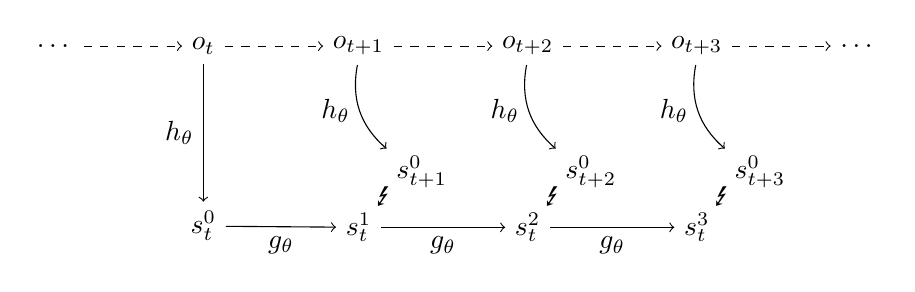
\begin{tikzpicture}[node distance=1.25]
        \node (ot) {$o_t$};
        \node [left = of ot] (otm1) {$\dots$};
        \node [right = of ot] (otp1) {$o_{t+1}$};
        \node [right = of otp1] (otp2) {$o_{t+2}$};
        \node [right = of otp2] (otp3) {$o_{t+3}$};
        \node [right = of otp3] (otp4) {$\dots$};
        \draw [->, dashed] (otm1) -- (ot);
        \draw [->, dashed] (ot) -- (otp1);
        \draw [->, dashed] (otp1) -- (otp2);
        \draw [->, dashed] (otp2) -- (otp3);
        \draw [->, dashed] (otp3) -- (otp4);

        \node [below = 1.75 of ot] (s0) {$s^0_t$};
        \node [below = 1.75 of otp1] (s1) {$s^1_t$};
        \node [below = 1.75 of otp2] (s2) {$s^2_t$};
        \node [below = 1.75 of otp3] (s3) {$s^3_t$};

        \draw [->] (ot) -- node [left] {$h_\theta$} (s0);
        \draw [->] (s0) -- node [below] {$g_\theta$} (s1);
        \draw [->] (s1) -- node [below] {$g_\theta$} (s2);
        \draw [->] (s2) -- node [below] {$g_\theta$} (s3);

        \node [above right = 0.1 of s1] (nots1) {$s^0_{t+1}$};
        \node [above right = -0.25 of s1] {\Lightning};
        \node [above right = 0.1 of s2] (nots2) {$s^0_{t+2}$};
        \node [above right = -0.25 of s2] {\Lightning};
        \node [above right = 0.1 of s3] (nots3) {$s^0_{t+3}$};
        \node [above right = -0.25 of s3] {\Lightning};

        \draw [->] (otp1) edge [bend right] node [left] {$h_\theta$} (nots1);
        \draw [->] (otp2) edge [bend right] node [left] {$h_\theta$} (nots2);
        \draw [->] (otp3) edge [bend right] node [left] {$h_\theta$} (nots3);
    \end{tikzpicture}
    \caption{Visualization of the discrepancy between state outputs of the dynamics function $g_\theta$ and representation function $h_\theta$.}
    \label{fig:consistency_loss}
\end{figure}

While the existence of multiple state formats may not be inherently destructive, and has been suggested to provide some benefits for the agent's understanding of the environment, we believe it can cause several problems. The most obvious of which is the need for the dynamics and prediction functions to learn how to use each of the different representations for the same estimates. If instead, $h_\theta$ and $g_\theta$ agree on a unified state format, this problem can be avoided. A more subtle but potentially more significant issue becomes apparent when we inspect MuZero's learning process. The functions are unrolled for $K$ timesteps across a given trajectory, and losses are computed for each timestep $k \in \{0, ..., K\}$. This means that $g_\theta$ and $f_\theta$ are trained on any state format that is produced by $g_\theta$ after up to $K$ iterations. For any further iterations, accuracy may degenerate. Depending on the search policy, it is not unlikely for the planning depth to become larger than $K$. In fact, the hyperparameters used for the original MuZero experiments have a small $K=5$ unroll depth for training, while at the same time using $50$ or even $800$ simulations for tree construction during planning, which can easily result in branches that are longer than $K$. By enforcing a consistent state representation, we may be able to mitigate the degeneration of performance for long planning branches.

We implement our change by continuously adjusting $\theta$ so that output $s^k_t$ of the dynamics function is close to output $s^0_{t+k}$ of the representation function. For example, we can perform gradient descent on the mean squared error between the state vectors. Mathematically, we express the consistency loss as $l^c(s^0_{t+k}, s^k_t)$, leading to an overall loss of
\begin{equation*}
    l_t(\theta) = \sum^K_{k=0} \left(l^r(u_{t+k}, r_t^k) + l^v(z_{t+k}, v_t^k) + l^p(\pi_{t+k}, \policy_t^k) + l^c(s^0_{t+k}, s^k_t) + c||\theta||^2\right).
\end{equation*}
Note that we treat the first parameter of $l^c$, $s^0_{t+k}$, as a constant, meaning the loss is not propagated directly to the representation function. Doing so would encourage $h_\theta$ and $g_\theta$ to always produce the same state outputs, regardless of the input. As a bonus, by only propagating the error through $s_t^k$ instead, the model is forced to maintain relevant information to predict subsequent states even in environments with sparse rewards, similar to the reconstruction loss from our previous proposal.
\section{Experiments}

\subsection{Results}

\begin{frame}[fragile]{Reconstruction Function}
    \begin{figure}
        \centering
        \begin{tikzpicture}[yscale=0.6, xscale=0.6,
                            define rgb/.code={\definecolor{mycolor}{RGB}{#1}},
                            rgb color/.style={define rgb={#1},mycolor}]
            \begin{axis}[
                title = CartPole-v1,
                axis lines = left,
                xlabel = Training steps,
                ylabel = Total reward,
                no markers,
                table/col sep = comma,
                legend cell align=left,
                legend pos=south east,
                legend style={draw=none},
                xmin=0,
                xmax=10000,
                grid=major,
            ]
                \addplot[black] table [
                    x = training_step,
                    y = reward,
                ] {results/default/CartPole-v1/lr0.0.csv};
                \addlegendentry{MuZero};

                \addplot[rgb color={32, 32, 180}] table [
                    x = training_step,
                    y = reward,
                ] {results/reconstruction/CartPole-v1/lr0.5.csv};
                \addlegendentry{$\frac{1}{2}l^g$};

                \addplot[rgb color={128, 128, 255}] table [
                    x = training_step,
                    y = reward,
                ] {results/reconstruction/CartPole-v1/lr1.0.csv};
                \addlegendentry{$l^g$};
            \end{axis}
        \end{tikzpicture}
        \begin{tikzpicture}[yscale=0.6, xscale=0.6,
                            define rgb/.code={\definecolor{mycolor}{RGB}{#1}},
                            rgb color/.style={define rgb={#1},mycolor}]
            \begin{axis}[
                title = LunarLander-v2,
                axis lines = left,
                xlabel = Training steps,
                ylabel = Total reward,
                no markers,
                table/col sep = comma,
                legend cell align=left,
                legend pos=south east,
                legend style={draw=none},
                xmin=0,
                xmax=30000,
                grid=major,
            ]
                \addplot[black] table [
                    x = training_step,
                    y = reward,
                ] {results/default/LunarLander-v2/lr0.0.csv};
                \addlegendentry{MuZero};

                \addplot[rgb color={32, 32, 180}] table [
                    x = training_step,
                    y = reward,
                ] {results/reconstruction/LunarLander-v2/lr0.5.csv};
                \addlegendentry{$\frac{1}{2}l^g$};

                \addplot[rgb color={128, 128, 255}] table [
                    x = training_step,
                    y = reward,
                ] {results/reconstruction/LunarLander-v2/lr1.0.csv};
                \addlegendentry{$l^g$};
            \end{axis}
        \end{tikzpicture}
        \caption{Total episode reward comparison of agents using the reconstruction loss term ($l^g$) and the default MuZero agent in the CartPole-v1 and LunarLander-v2 environments, averaged across 32 and 25 runs, respectively.}
        \label{fig:reconstruction_results}
    \end{figure}
\end{frame}

\begin{frame}[fragile]{Consistency Loss}
    \begin{figure}
        \centering
        \begin{tikzpicture}[yscale=0.6, xscale=0.6,
                            define rgb/.code={\definecolor{mycolor}{RGB}{#1}},
                            rgb color/.style={define rgb={#1},mycolor}]
            \begin{axis}[
                title = CartPole-v1,
                axis lines = left,
                xlabel = Training steps,
                ylabel = Total reward,
                no markers,
                table/col sep = comma,
                legend cell align=left,
                legend pos=south east,
                legend style={draw=none},
                xmin=0,
                xmax=10000,
                grid=major,
            ]
                \addplot[black] table [
                    x = training_step,
                    y = reward,
                ] {results/default/CartPole-v1/lr0.0.csv};
                \addlegendentry{MuZero};

                \addplot[rgb color={32, 128, 32}] table [
                    x = training_step,
                    y = reward,
                ] {results/consistency/CartPole-v1/lr0.5.csv};
                \addlegendentry{$\frac{1}{2}l^c$};

                \addplot[rgb color={0, 255, 0}] table [
                    x = training_step,
                    y = reward,
                ] {results/consistency/CartPole-v1/lr1.0.csv};
                \addlegendentry{$l^c$};
            \end{axis}
        \end{tikzpicture}
        \begin{tikzpicture}[yscale=0.6, xscale=0.6,
                            define rgb/.code={\definecolor{mycolor}{RGB}{#1}},
                            rgb color/.style={define rgb={#1},mycolor}]
            \begin{axis}[
                title = LunarLander-v2,
                axis lines = left,
                xlabel = Training steps,
                ylabel = Total reward,
                no markers,
                table/col sep = comma,
                legend cell align=left,
                legend pos=south east,
                legend style={draw=none},
                xmin=0,
                xmax=30000,
                grid=major,
            ]
                \addplot[black] table [
                    x = training_step,
                    y = reward,
                ] {results/default/LunarLander-v2/lr0.0.csv};
                \addlegendentry{MuZero};

                \addplot[rgb color={32, 128, 32}] table [
                    x = training_step,
                    y = reward,
                ] {results/consistency/LunarLander-v2/lr0.5.csv};
                \addlegendentry{$\frac{1}{2}l^c$};

                \addplot[rgb color={0, 255, 0}] table [
                    x = training_step,
                    y = reward,
                ] {results/consistency/LunarLander-v2/lr1.0.csv};
                \addlegendentry{$l^c$};
            \end{axis}
        \end{tikzpicture}
        \caption{Total episode reward comparison of agents the consistency loss ($l^c$) and the default MuZero agent in the CartPole-v1 and LunarLander-v2 environments, averaged across 32 and 25 runs, respectively.}
        \label{fig:consistency_results}
    \end{figure}
\end{frame}

\begin{frame}[fragile]{Hybrid Method}
    \begin{figure}
        \centering
        \begin{tikzpicture}[yscale=0.6, xscale=0.6,
                            define rgb/.code={\definecolor{mycolor}{RGB}{#1}},
                            rgb color/.style={define rgb={#1},mycolor}]
            \begin{axis}[
                title = CartPole-v1,
                axis lines = left,
                xlabel = Training steps,
                ylabel = Total reward,
                no markers,
                table/col sep = comma,
                legend cell align=left,
                legend pos=south east,
                legend style={draw=none},
                xmin=0,
                xmax=10000,
                grid=major,
            ]
                \addplot[black] table [
                    x = training_step,
                    y = reward,
                ] {results/default/CartPole-v1/lr0.0.csv};
                \addlegendentry{MuZero};

                \addplot[rgb color={128, 128, 255}] table [
                    x = training_step,
                    y = reward,
                ] {results/reconstruction/CartPole-v1/lr1.0.csv};
                \addlegendentry{$l^g$};

                \addplot[rgb color={0, 128, 128}] table [
                    x = training_step,
                    y = reward,
                ] {results/hybrid/CartPole-v1/lr0.5.csv};
                \addlegendentry{$\frac{1}{2}l^g + \frac{1}{2}l^c$};

                \addplot[rgb color={0, 200, 200}] table [
                    x = training_step,
                    y = reward,
                ] {results/hybrid/CartPole-v1/lr1.0.csv};
                \addlegendentry{$l^g + l^c$};
            \end{axis}
        \end{tikzpicture}
        \begin{tikzpicture}[yscale=0.6, xscale=0.6,
                            define rgb/.code={\definecolor{mycolor}{RGB}{#1}},
                            rgb color/.style={define rgb={#1},mycolor}]
            \begin{axis}[
                title = LunarLander-v2,
                axis lines = left,
                xlabel = Training steps,
                ylabel = Total reward,
                no markers,
                table/col sep = comma,
                legend cell align=left,
                legend pos=south east,
                legend style={draw=none},
                xmin=0,
                xmax=30000,
                grid=major,
            ]
                \addplot[black] table [
                    x = training_step,
                    y = reward,
                ] {results/default/LunarLander-v2/lr0.0.csv};
                \addlegendentry{MuZero};

                \addplot[rgb color={128, 128, 255}] table [
                    x = training_step,
                    y = reward,
                ] {results/reconstruction/LunarLander-v2/lr1.0.csv};
                \addlegendentry{$l^g$};

                \addplot[rgb color={0, 128, 128}] table [
                    x = training_step,
                    y = reward,
                ] {results/hybrid/LunarLander-v2/lr0.5.csv};
                \addlegendentry{$\frac{1}{2}l^g + \frac{1}{2}l^c$};

                \addplot[rgb color={0, 200, 200}] table [
                    x = training_step,
                    y = reward,
                ] {results/hybrid/LunarLander-v2/lr1.0.csv};
                \addlegendentry{$l^g + l^c$};
            \end{axis}
        \end{tikzpicture}
        \caption{Total episode reward comparison of agents using both the reconstruction function loss ($l^g$) as well as the consistency loss term ($l^c$) simultaneously in the CartPole-v1 and LunarLander-v2 environments, averaged across 32 and 25 runs, respectively.}
        \label{fig:hybrid_results}
    \end{figure}
\end{frame}

\begin{frame}[fragile]{Pretrained Hybrid}
    \begin{figure}
        \centering
        \begin{tikzpicture}[yscale=0.6, xscale=0.6,
                            define rgb/.code={\definecolor{mycolor}{RGB}{#1}},
                            rgb color/.style={define rgb={#1},mycolor}]
            \begin{axis}[
                title = CartPole-v1,
                axis lines = left,
                xlabel = Training steps,
                ylabel = Total reward,
                no markers,
                table/col sep = comma,
                legend cell align=left,
                legend pos=south east,
                legend style={draw=none},
                xmin=0,
                xmax=10000,
                grid=major,
            ]
                \addplot[black] table [
                    x = training_step,
                    y = reward,
                ] {results/default/CartPole-v1/lr0.0.csv};
                \addlegendentry{MuZero};

                \addplot[rgb color={0, 200, 200}] table [
                    x = training_step,
                    y = reward,
                ] {results/hybrid/CartPole-v1/lr1.0.csv};
                \addlegendentry{$l^g + l^c$};

                \addplot[rgb color={220, 80, 80}] table [
                    x = training_step,
                    y = reward,
                ] {results/pretrained/CartPole-v1/lr1.0.csv};
                \addlegendentry{$l^g + l^c$ (pretrained)};
            \end{axis}
        \end{tikzpicture}
        \begin{tikzpicture}[yscale=0.6, xscale=0.6,
                            define rgb/.code={\definecolor{mycolor}{RGB}{#1}},
                            rgb color/.style={define rgb={#1},mycolor}]
            \begin{axis}[
                title = LunarLander-v2,
                axis lines = left,
                xlabel = Training steps,
                ylabel = Total reward,
                no markers,
                table/col sep = comma,
                legend cell align=left,
                legend pos=south east,
                legend style={draw=none},
                xmin=0,
                xmax=30000,
                grid=major,
            ]
                \addplot[black] table [
                    x = training_step,
                    y = reward,
                ] {results/default/LunarLander-v2/lr0.0.csv};
                \addlegendentry{MuZero};

                \addplot[rgb color={0, 200, 200}] table [
                    x = training_step,
                    y = reward,
                ] {results/hybrid/LunarLander-v2/lr1.0.csv};
                \addlegendentry{$l^g + l^c$};

                \addplot[rgb color={220, 80, 80}] table [
                    x = training_step,
                    y = reward,
                ] {results/pretrained/LunarLander-v2/lr1.0.csv};
                \addlegendentry{$l^g + l^c$ (pretrained)};
            \end{axis}
        \end{tikzpicture}
        \caption{Total episode reward comparison of agents using both the reconstruction function loss ($l^g$) as well as the consistency loss term ($l^c$) simultaneously as a pretrained and non-pretrained variant in the CartPole-v1 and LunarLander-v2 environments, averaged across 32 and 25 runs, respectively.}
        \label{fig:pretrained_results}
    \end{figure}
\end{frame}

\begin{frame}{Numeric Comparison}
    \begin{table}
        \centering
        \begin{tabular}{|l||c|c|}
            \hline
            & CartPole-v1 & LunarLander-v2 \\
            \hline \hline
            MuZero & $281.42 \pm 162.48$ & $-34.86 \pm 92.87$ \\
            \hline
            $l^g$ & $375.85 \pm 149.38$ & $42.67 \pm 132.59$\\
            \hline
            $l^c$ & $296.45 \pm 174.55$ & $32.17 \pm 145.90$ \\
            \hline
            $l^g + l^c$ & $\mathbf{410.59 \pm 130.71}$ & $100.46 \pm 123.82$ \\
            \hline
            $l^g + l^c$ (pretrained) & $335.72 \pm 162.49$ & $\mathbf{104.99 \pm 116.67}$ \\
            \hline
        \end{tabular}
        \caption{Comparison of the default MuZero algorithm and the modifications described in this thesis on the CartPole-v1 and LunarLander-v2 environments. The terms $l^g$ and $l^c$ stand for the addition of a reconstruction or consistency loss, respectively. The results show the mean and standard deviation of the total reward for the final $500$ training steps across all test runs.}
        \label{tab:results_table}
    \end{table}
\end{frame}


\section{Conclusion}

\bibliography{bibliography}
\bibliographystyle{apalike}

\end{document}